% This file was created with tikzplotlib v0.10.1.
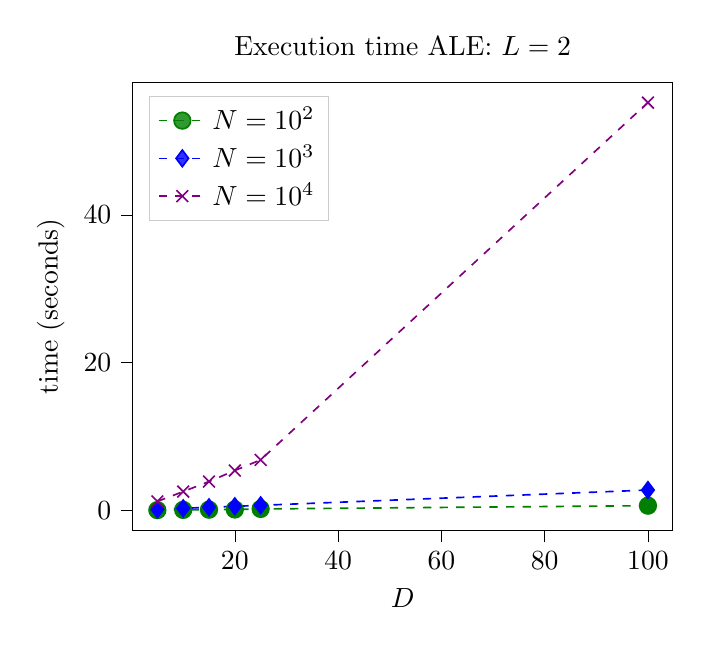
\begin{tikzpicture}

\definecolor{darkgray176}{RGB}{176,176,176}
\definecolor{green01270}{RGB}{0,127,0}
\definecolor{lightgray204}{RGB}{204,204,204}
\definecolor{purple}{RGB}{128,0,128}

\begin{axis}[
legend cell align={left},
legend style={
  fill opacity=0.8,
  draw opacity=1,
  text opacity=1,
  at={(0.03,0.97)},
  anchor=north west,
  draw=lightgray204
},
tick align=outside,
tick pos=left,
title={Execution time ALE: \(\displaystyle L=2\)},
x grid style={darkgray176},
xlabel={\(\displaystyle D\)},
xmin=0.25, xmax=104.75,
xtick style={color=black},
y grid style={darkgray176},
ylabel={time (seconds)},
ymin=-2.73388298709979, ymax=57.999057591099,
ytick style={color=black}
]
\addplot [semithick, green01270, dashed, mark=*, mark size=3, mark options={solid}]
table {%
5 0.026705265045166
10 0.0574851036071777
15 0.0858516693115234
20 0.112214326858521
25 0.184911131858826
100 0.628105640411377
};
\addlegendentry{$N=10^2$}
\addplot [semithick, blue, dashed, mark=diamond*, mark size=3, mark options={solid}]
table {%
5 0.127141833305359
10 0.271587371826172
15 0.413034200668335
20 0.54520583152771
25 0.675822854042053
100 2.74792742729187
};
\addlegendentry{$N=10^3$}
\addplot [semithick, purple, dashed, mark=x, mark size=3, mark options={solid}]
table {%
5 1.20529174804688
10 2.53928112983704
15 3.89853239059448
20 5.39064311981201
25 6.83541965484619
100 55.238468170166
};
\addlegendentry{$N=10^4$}
\end{axis}

\end{tikzpicture}
